

%----------------------------------------------------------------------------------------
\section{FAIMS 3.0}

\begin{sectionframe} % Custom environment required for section slides
	\frametitle{FAIMS 3.0}
	\framesubtitle{Report on current development}



\vfill
\begin{columns}[T]

\begin{column}{0.55\textwidth}
\centering
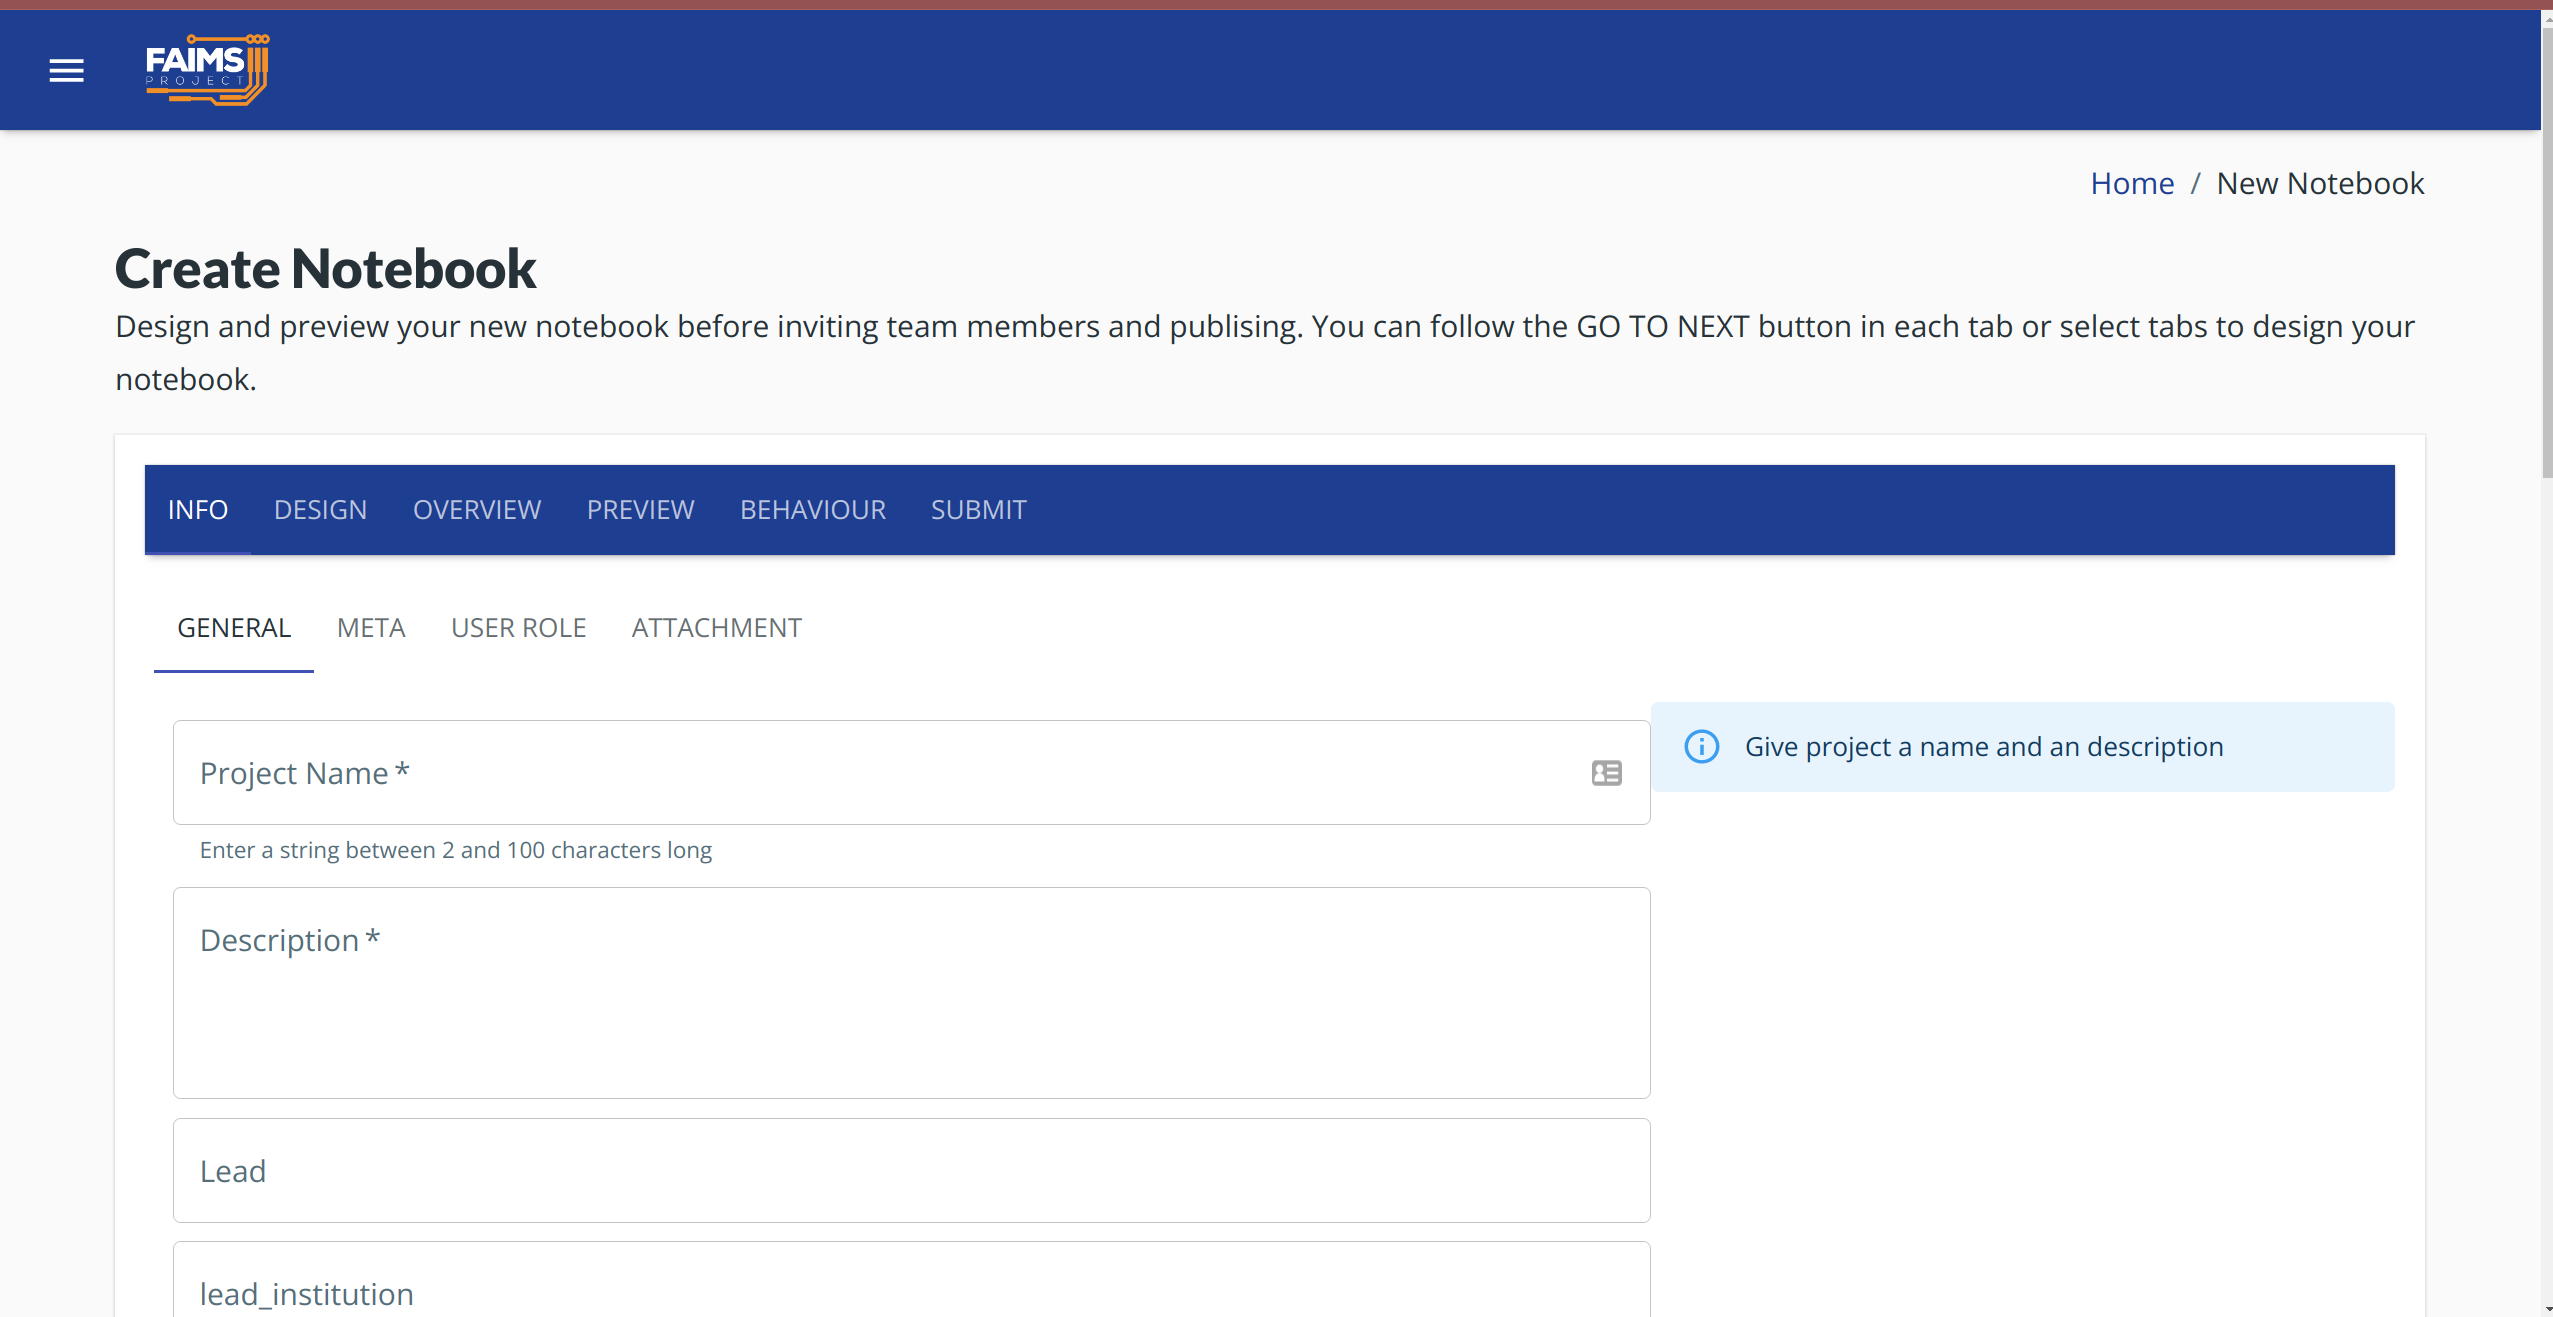
\includegraphics[width=\textwidth]{Images/Screenshot_20211209_123600_Selection_001.png}
\end{column}
\begin{column}{0.35\textwidth}
\centering
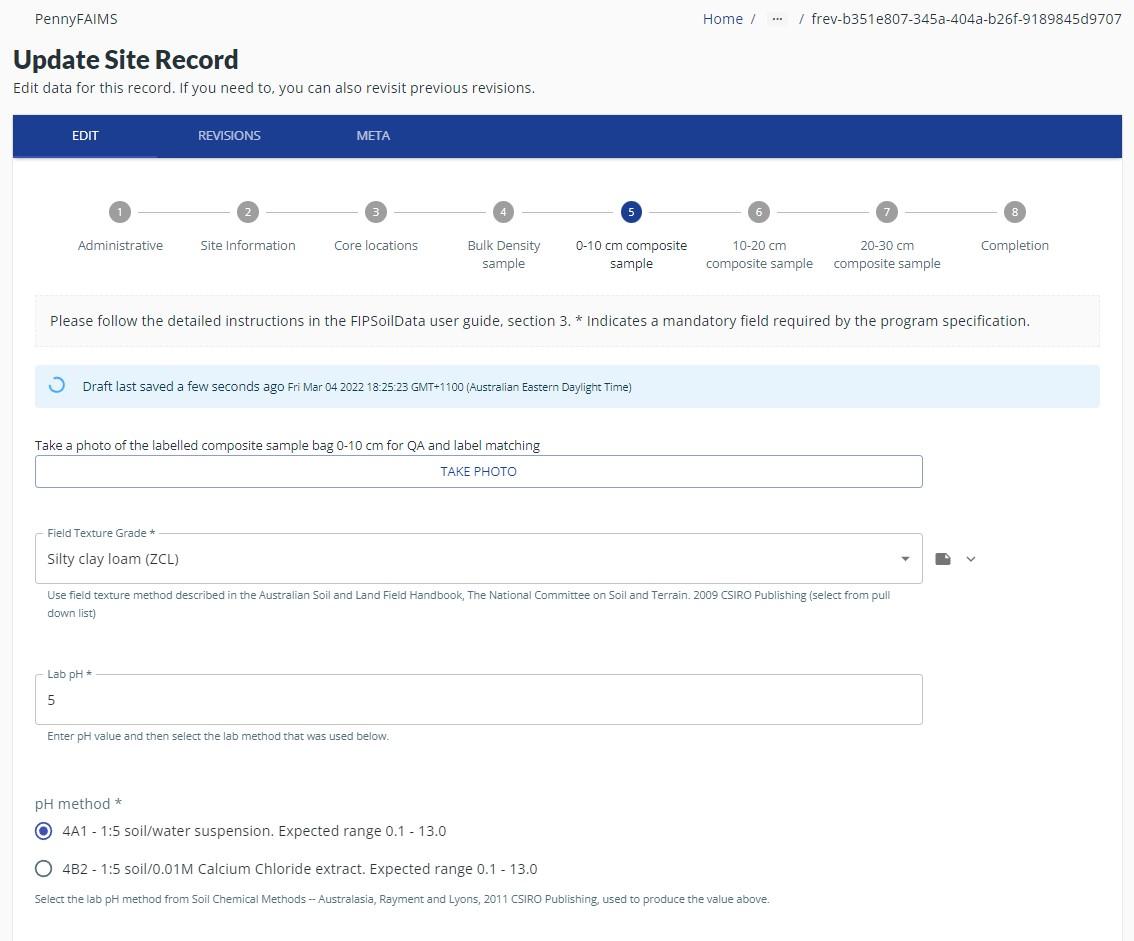
\includegraphics[width=\textwidth]{Images/Screenshot 2022-03-04 182606.jpg} 
\end{column}

\end{columns}

% 	This is on another line
\end{sectionframe}

%----------------------------------------------------------------------------------------

\begin{frame}{FAIMS 3.0 overview}

\begin{itemize}
    \item Ground up rebuild with a modern architecture (Javascript using NodeJS and Couch/Pouch DB);
    \item Cross-platform data collection (Android/iOS/web-native); 
    \item Improved interoperability with other software (for data 'round trips' with processing / analysis software); and
    \item GUI for electronic field notebook creation (facilitating self-service customisation).
\end{itemize}

\end{frame}
%----------------------------------------------------------------------------------------

\begin{frame}{Where are we now?}
    \begin{itemize}
        \item FAIMS v2.6 is depreciated but currently supporting legacy users.
        \item The FAIMS team did CSIRO ON Prime in 2016, completing 70+ interviews with clients / potential clients.
        \item A high-level technical plan for FAIMS v3.0 won a US design prize in 2017 \parencite{Bureau_of_Reclamation2017-xl}.
        \item ARDC Platforms announced a major co-investment in late 2019 to rebuild FAIMS using modern components.
        \item We released a private alpha of FAIMS3 in late 2021.
        \item We are currently supporting a major CSIRO initiative with data being collected in an early build of FAIMS3 as we speak.
    \end{itemize}
\end{frame}
%----------------------------------------------------------------------------------------


\begin{frame}{Opportunities and challenges}
    \begin{itemize}
        \item Useful research-specific features of FAIMS v2.6 to be retained.
        \item Android-only hindered uptake; cross-platform support required.
        \item Lack of self-service customisation / deployment hindered uptake.
        \item Users want to be able to edit data on the desktop or online, then have that data available for further editing in the field (data `round-trip' outside of the application).
        \item Users want more options for accessing / exporting data on-demand.
        \item Users want to be able to use the platform for sensitive data. 
        \item Improved scalability needed (application performance; server-to-server synchronisation)
        \item Enterprise features (orchestration, user management, reporting, branding, SSO, etc.) needed for eventual COSS \textbf{product} to support sustainability (underlying software \textbf{project} will remain OS).
    \end{itemize}
\end{frame}
%----------------------------------------------------------------------------------------

\begin{frame}{FAIMS 3.0 development approach}
Technical elaboration in 2020 produced an \href{https://zenodo.org/record/4616766}{Elaboration Report}; our approach includes:
    \begin{itemize}
        \item NODE.JS
        \item NoSQL datastore (Apache CouchDB / PouchDB)
        \item APIs for data interactions (CouchDB)
        \item Progressive JS Single Page Application wrapped in Native code
for cross-platform support using Capacitor
        \item JSON Forms
        \item Javascript mapping library (OpenLayers)
        \item Plugin architecture

    \end{itemize}
\end{frame}
%----------------------------------------------------------------------------------------


\begin{frame}{FAIMS 3.0 development approach}
Other planned, but not yet elaborated, technical capabilities include:
    \begin{itemize}
        \item Web application to provide GUI to produce definition files
        \item 'Real' user management and security
        \item Interoperability with Cloudstor, EOSC nodes, ELNs, domain repositories (data `round-trip' export-modify-import)
        \item Device support (cameras, printers, instruments, etc.)
        \item Offline mapping
        \item Audio/video management
    \end{itemize}
\end{frame}

%----------------------------------------------------------------------------------------

\begin{frame}
    \frametitle{FAIMS 3.0 development progress}
    \framesubtitle{Development Progress}        
        \begin{itemize}
            \item \href{https://docs.google.com/document/d/13eTN8jhJa3Pgs9GOdo7r4jtIQcskNo7ikxJcBDBKHzw/edit}{Technical Elaboration Report} was approved in February. This established the proof-of-concept for FAIMS3. 
          \item \href{https://github.com/FAIMS/FAIMS3/releases/tag/v0.1.0-alpha}{Alpha prototype} was released on 11 June 2021.  
          \item Alpha prototype passed \href{https://doi.org/10.5281/zenodo.5030772}{user-acceptance testing} on 15 June 2021.
        \item FAIMS3 code has been licensed under the \href{https://www.apache.org/licenses/LICENSE-2.0}{Apache2} license, a Developer Contribution agreement is being applied to all code affirming the license. 
        \item The FAIMS3 repository is now public on \href{https://github.com/FAIMS/FAIMS3}{GitHub}.
        \item FAIMS3 Beta development commenced on 5 July 2021 and will conclude 1 November 2021. 
        \item CSIRO supported extra development Jan 2022 -- July 2022 extra of ARDC funding for DAWE's Pilot Soils Monitoring and Incentives Program.

    \end{itemize}



\end{frame} 